\section{Methods}
\subsection{Phase diagram generation}\label{sec:cem}
Gibbs phase stability states that a globally stable equilibrium state can be obtained by constructing (lower) convex hull of energy over composition~\cite{OryllCEM,SoftMatterCEM}. 
A phase diagram can be determined by applying Gibbs stability criteria of energy landscape~\cite{GibbsCriteria1} using the convex envelope method~(CEM) introduced in~\cite{OryllCEM,SoftMatterCEM}.
According to Gibbs rules, stable compositions lie on the convex hull of energy landscape while unstable compositions lie above.
The CEM is generic and can be applied to any given energy function form. 
Two forms of energy functions are evaluated: polynomial and Flory-Huggins.
The later is used to study the multi-component organic blend system and is defined using the generalized form for an \(N\) component system given by~\Cref{eq:FH}. 
\begin{equation}\label{eq:FH}
    f_{\text{FH}} = \sum_{i=1}^{N}  \frac{1}{M_i} \phi_{i}\lnn{\phi_i} + \sum_{i=1}^{N}\sum_{j(\neq i)=1}^{N}\phi_i \phi_j \chi_{ij}
\end{equation}
where \(\phi\) is composition defined in terms of volume fraction , \(N\) is total number of components in the mixture, \(\chi_{ij}\) are Flory-Huggins interaction parameters between components \(i,j\) and \(M_i\) is degree of polymerization of \(i^{th}\) compound. 

A step-by-step procedure of CEM is described below and an example is shown in~\Cref{fig:workflow} for a three component system (i.e. \(N=3\)).
\begin{enumerate}\label{algo:cem}
    \item[Input:] Free energy function, desired mesh size
    \item[1.] \textbf{Grid generation:} Create a grid \(G\) using an user-defined mesh size $N_{\phi}$ (in terms of number of points per component/dimension) as an n-dimensional hyperplane of compositions (volume fractions \(\{\phi_i\}_{i=1}^{n}\)).
    \item[2.] \textbf{Compute free energy landscape:} Evaluate free energy at each point in \(G\). This results in a (discrete) energy landscape. 
    \item[3.] \textbf{Compute convex envelope:} Compute the convex hull of energy landscape. 
    \item[4.] \textbf{Lower convex hull}: Obtain a lower convex hull~\footnote{Given a energy landscape as a set of points and a height function (energy) , one can obtain the lower convex hull by first adding a point at infinity height to the set and then excluding the simplices that connect to it.} and project it to \(G\) by simply looking up the vertex indices resulting in a mesh of \(G\). 
    The outcome from this step is the projected lower hull, \(G_l\), where vertices corresponds to the points in \(G\).
    \item[5.] \textbf{Compute phase labels:} For each simplex in the mesh $G_l$, assign a phase label based on the number of connected components (as described in~\cite{SoftMatterCEM}). 
    An user defined threshold \(\Delta\) is used to compute adjacency matrix which in turn is used to compute number of connected components.
    \item[Output:] Phase diagram represented as $G_l$ with the phase label assigned to each simplex. 
\end{enumerate}

\begin{figure}[h]
    \centering
    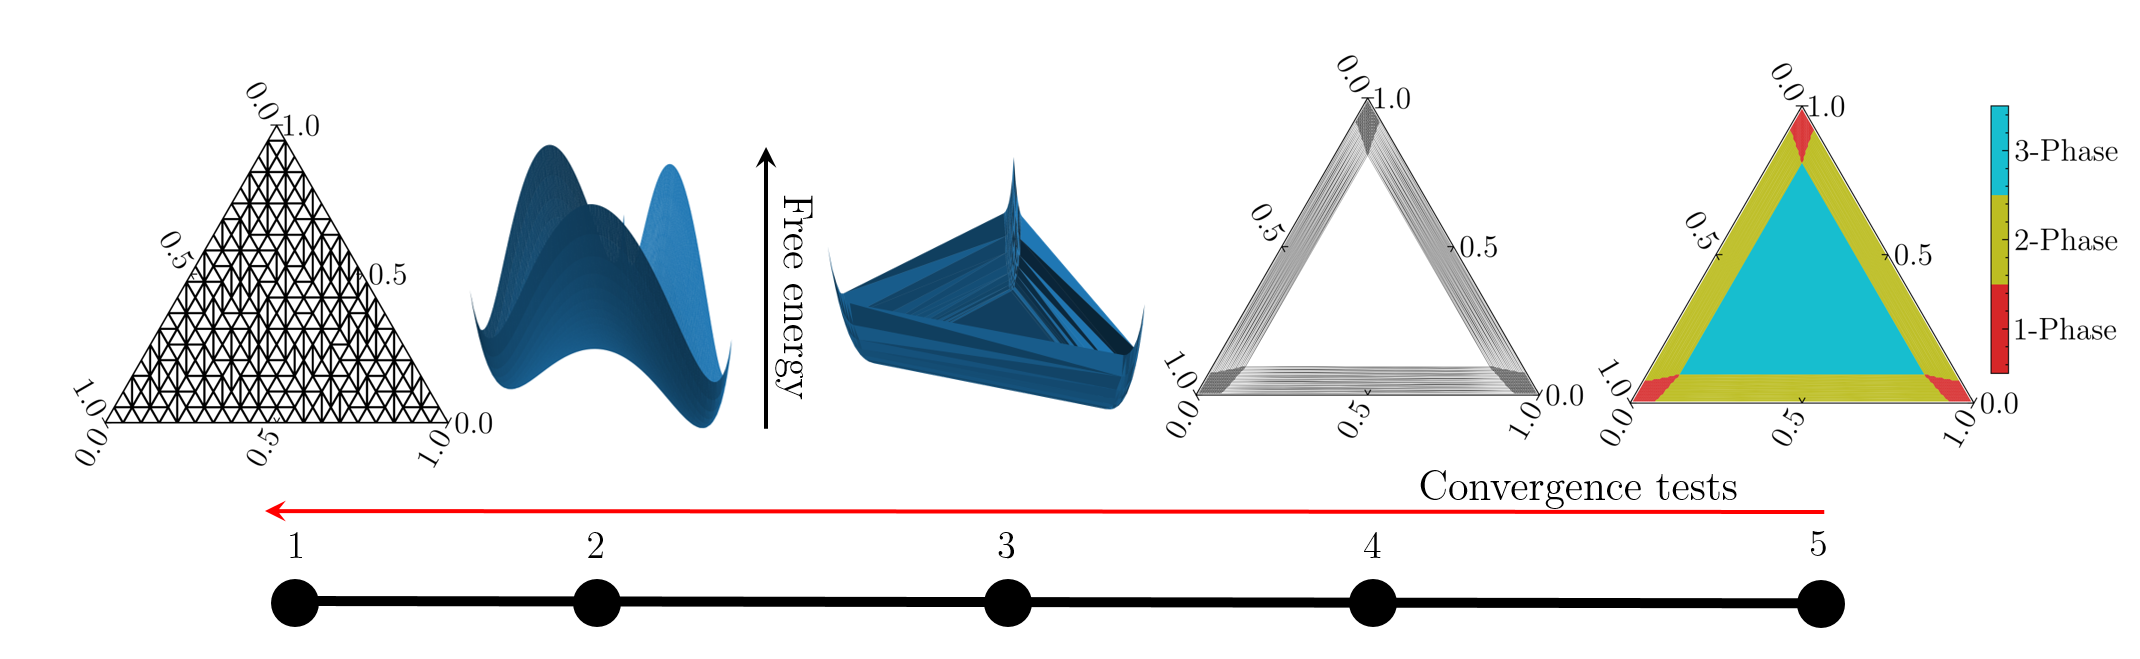
\includegraphics[width=\textwidth]{Chapter-4/figures/CEM_workflow.png}
    \caption{Convex envelope method visualized as a step-by-step process (1-5) with the series of tests performed. The red arrows depict where the tests can be performed and iterated until convergence, if required.}
    \label{fig:workflow}
\end{figure}

Two representations of phase diagrams are used:
The first representation corresponds to the output from~\Cref{algo:cem} and is referred as simplex-indexed set representation. 
The second representation is a a set indexed on the initial uniform grid $G$ (step 1 of~\Cref{algo:cem}), and is referred as a grid-indexed set representation.
The advantage of the second representation is the fixed size that ease the distance calculation. 
The grid-indexed representation is obtained from the simplex-indexed representation by assigning the phase label for each point in the grid by mapping it to the corresponding simplex in the convex envelope. 
The grid-indexed representation is used for the data analysis in~\Cref{sec:pipeline} and differentiate it from its simplex-indexed representation by a change of color-code while visualizing the phase diagram.
